\definecolor{mygreen}{rgb}{0,0.6,0}
\definecolor{mygray}{rgb}{0.5,0.5,0.5}
\definecolor{mymauve}{rgb}{0.58,0,0.82}

%%%%%%%%%%%%%%%%%%%%%%%%%%%%%%%%%%%%%%%%%%%%%%%%%%%%%%%%%%%%%%%%%%%%%%%%%%%%%
% parámetros para configurar el formato del código en los entornos lstlisting
%%%%%%%%%%%%%%%%%%%%%%%%%%%%%%%%%%%%%%%%%%%%%%%%%%%%%%%%%%%%%%%%%%%%%%%%%%%%%
\lstset{ %
  backgroundcolor=\color{white},   % choose the background color; you must add \usepackage{color} or \usepackage{xcolor}
  basicstyle=\footnotesize,        % the size of the fonts that are used for the code
  breakatwhitespace=false,         % sets if automatic breaks should only happen at whitespace
  breaklines=true,                 % sets automatic line breaking
  captionpos=b,                    % sets the caption-position to bottom
  commentstyle=\color{mygreen},    % comment style
  deletekeywords={...},            % if you want to delete keywords from the given language
  %escapeinside={\%*}{*)},          % if you want to add LaTeX within your code
  %extendedchars=true,              % lets you use non-ASCII characters; for 8-bits encodings only, does not work with UTF-8
  %frame=single,	                % adds a frame around the code
  keepspaces=true,                 % keeps spaces in text, useful for keeping indentation of code (possibly needs columns=flexible)
  keywordstyle=\color{blue},       % keyword style
  language=[ANSI]C,                % the language of the code
  %otherkeywords={*,...},           % if you want to add more keywords to the set
  numbers=left,                    % where to put the line-numbers; possible values are (none, left, right)
  numbersep=5pt,                   % how far the line-numbers are from the code
  numberstyle=\tiny\color{mygray}, % the style that is used for the line-numbers
  rulecolor=\color{black},         % if not set, the frame-color may be changed on line-breaks within not-black text (e.g. comments (green here))
  showspaces=false,                % show spaces everywhere adding particular underscores; it overrides 'showstringspaces'
  showstringspaces=false,          % underline spaces within strings only
  showtabs=false,                  % show tabs within strings adding particular underscores
  stepnumber=1,                    % the step between two line-numbers. If it's 1, each line will be numbered
  stringstyle=\color{mymauve},     % string literal style
  tabsize=2,	                   % sets default tabsize to 2 spaces
  title=\lstname,                  % show the filename of files included with \lstinputlisting; also try caption instead of title
  morecomment=[s]{/*}{*/}
}


\chapter{Diseño e Implementación} % Main chapter title

\label{Chapter3} % Change X to a consecutive number; for referencing this chapter elsewhere, use \ref{ChapterX}


En este capítulo se explican con detalle todo los elementos que componen al sistema y los criterios utilizados para su desarrollo. Se parte de una breve descripción de la estructura del sistema, pasando por el desarrollo de los módulos de hardware y se concluye con la implementación del software.


\section{Estructura general del sistema}
Con el objetivo de lograr un sistema adaptable y escalable se optó por realizar un diseño modular. Este diseño consiste en tres tipos de módulos o etapas: el módulo principal, los módulos adicionales y la interfaz de usuario. La figura \ref{fig:BloquesGral} indica en forma general la estructura del sistema y el modo en que los módulos están conectados entre sí.


\begin{figure}[ht]
	\centering
	\includegraphics[scale=0.5]{./Figures/BloquesGral.pdf}
	\caption{Diagrama en bloques del sistema.}
	\label{fig:BloquesGral}
\end{figure}

\subsection{Módulo principal}
El módulo principal es la base del sistema, allí se encuentra el núcleo de procesamiento, la etapa de comunicación con la interfaz de usuario, el servidor web de la misma y los puertos de conexión con los módulos adicionales. Estos puertos de conexión son los encargados de capturar las señales provenientes de los módulos adicionales, tanto en forma analógica como digital. Además, son capaces de generar señales analógicas y digitales y proveer de alimentación a los módulos adicionales.
Una característica importante de estos puertos de conexión es que se encuentran aislados eléctricamente uno del otro para poder trabajar con equipos no aislados y únicamente se  comunican con el núcleo de procesamiento mediante una interfaz optoaislada.

\subsection{Módulos adicionales}
Los módulos adicionales cumplen las funciones de conectar y adaptar las señales entre los puertos del módulo principal y el equipo bajo prueba. Estos módulos se diseñan específicamente para cada tipo o familia de productos. Gracias a esta estructura modular se puede adaptar el sistema para realizar distintas pruebas con pocos cambios de hardware.
Al momento se desarrollaron dos módulos adicionales, uno para prueba de temporizadores y otro para la prueba de salida de drivers.

\subsection{Interfaz de Usuario}
La interfaz de usuario es el medio por el cual se controla al sistema. Se desarrolló de forma que pueda ejecutarse en cualquier plataforma que tenga un navegador web y esté conectada a la misma red que el módulo principal. Por ejemplo, se puede ejecutar desde una tablet, notebook o celular y con solo ingresar el IP del sistema de pruebas se tiene acceso al panel de control donde se puede seleccionar la prueba a realizar, configurar los parámetros, ejecutar las pruebas y visualizar los resultados.

\section{Desarrollo de hardware del módulo principal}

El módulo principal, como se mencionó anteriormente, posee el núcleo de procesamiento implementado con una placa de desarrollo EDU-CIAA, un módulo de comunicación WIFI ESP-01 para la interfaz de usuario y los puertos de conexión con los módulos adicionales. En la figura \ref{fig:BloquesPrincipal} se presenta un diagrama en bloques del módulo principal cuyos elementos serán detallados a continuación.

\begin{figure}[H]
	\centering
	\includegraphics[width=1\textwidth]{./Figures/bloquesPrincipal.pdf}
	\caption{Diagrama en bloques del módulo principal.}
	\label{fig:BloquesPrincipal}
\end{figure}



\subsection{Placa de desarrollo EDU-CIAA}

El uso de la placa de desarrollo EDU-CIAA como núcleo de procesamiento fue uno de los requerimientos establecidos al inicio del proyecto. Esta decisión se basó principalmente en que la EDU-CAA es la plataforma sobre la que más se trabajó durante la especialización y se dispone de gran variedad de recursos de software y soporte por parte de la comunidad. 
Respecto al hardware, la placa dispone un procesador LPC4337 con dos núcleos asimétricos, un Cortex M4 y un Cortex M0, trabajando a 208 Mhz y un amplio abanico de interfaces de comunicación como ser bus I2C, SPI, USB, CAN y varias UARTs. 


\subsection{Puertos de conexión}
\label{sec:puertos}

Los puertos de conexión son las piezas de hardware que más trabajo requirieron en su diseño. Fue necesario desarrollar dos esquemas preliminares de hardware a causa de que las primeras pruebas que se realizaron no fueron exitosas. Esto se debió a que el diseño no contemplaba el hecho de que muchos drivers de LEDs no están aislados entre entrada y salida, impidiendo así el uso de una masa común entre los distintos puertos de conexión. Siendo imposible solucionar esto sin alterar la topología del circuito, se optó por un esquema de puertos opto-aislados. La figura \ref{fig:BloquesPuerto} representa en un esquema de bloques el circuito de un puerto de conexión donde se puede apreciar que cada puerto dispone de un microcontrolador de la familia STM32, en particular para el desarrollo se eligió un módulo Bluepill basado en el microcontrolador STM32F108C8T6 con núcleo Cortex M3. Este microcontrolador cumple las siguientes funciones:

\begin{itemize}
	\item Comunicación mediante UART opto-aislada con la EDU-CIAA.
	\item Capturar el estado de las 3 entradas digitales del puerto.
	\item Muestreo de las 2 entradas analógicas del puerto.
	\item Comunicación con el conversor digital-analógico de la salida analógica 0-10v.
	\item Generar las señales de las 3 salidas digitales del puerto y activar el relay de alimentación de 220VAC.
\end{itemize}

\begin{figure}[ht]
	\centering
	\includegraphics[width=1\textwidth]{./Figures/BloquesPuerto.pdf}
	\caption{Diagrama en bloques de un puerto de conexión.}
	\label{fig:BloquesPuerto}
\end{figure}


\subsection{Interfaz UART opto-aislada}
	
Para el diseño de la interfaz UART opto-aislada se tuvieron en cuenta los requerimientos de cantidad de canales analógico a digital y digital a analógico, la velocidad de muestreo y el número de entradas y salidas digitales, que en forma indirecta establecen la velocidad de comunicación mínima que debe poseer la interfaz UART opto-aislada entre los puertos y la EDU-CIAA.
También fue necesario establecer un protocolo para empaquetar los datos e identificar a qué puerto corresponde cada paquete de datos.
El protocolo diseñado consiste en un protocolo maestro-esclavos donde un maestro, en este caso la EDU-CIAA, inicia la comunicación con un esclavo enviando una trama de 5 bytes, como lo indica la figura \ref{fig:TramaMS}, que a través de la UART opto-aislada llega a todos los puertos.

\begin{figure}[H]
	\centering
	\includegraphics[width=1\textwidth]{./Figures/TramaMS.pdf}
	\caption{Estructura de una trama de datos de maestro a esclavo.}
	\label{fig:TramaMS}
\end{figure}

A continuación cada esclavo, es decir cada uno de los puertos, captura la trama y obtiene la dirección correspondiente a la trama recibida y la compara con la propia. Solo el esclavo con la misma dirección debe responder al maestro mediante una trama de 4 bytes con la estructura que se indica en la figura \ref{fig:TramaSM}.

\begin{figure}[H]
	\centering
	\includegraphics[width=1\textwidth]{./Figures/TramaSM.pdf}
	\caption{Estructura de una trama de datos de esclavo a maestro.}
	\label{fig:TramaSM}
\end{figure}

Una vez establecido el protocolo donde se deben transmitir 5 bytes de maestro a esclavo y 4 bytes de esclavo a maestro en configuración full-duplex, y teniendo en cuenta que en el listado de requerimientos se establecio una taza de refresco de mil veces por segundo por cada uno de los seis puertos, se calculó una velocidad de comunicación mínima requerida de 30 KB/s. Luego se escogió la velocidad estándar más cercana para un puerto UART, siendo ésta 460800 Kb/s excede ampliamente lo minimo requerido y deja espacio para futuras expansiones.

Para la selección de los opto acopladores, se evaluaron algunas alternativas disponibles en el mercado local. La tabla \ref{tab:Optos} resume las características principales de los mismos donde se puede destacar al tiempo de respuesta como el factor limitante. 
Utilizando como criterio de diseño que el tiempo de respuesta del optoacoplador debe ser 10 veces menor que el tiempo de un bit para lograr una salida aceptable, significa que para lograr una velocidad de 460800 Kb/s se requiere un tiempo de respuesta menor a 217 ns. Por lo tanto en la tabla \ref{tab:Optos} se puede observar que la mejor opción para la aplicación es el optoacoplador 6N137 debido a que es el único capaz de trabajar a la velocidad de 460800 Kb/s requerida.

	\begin{table}[h]
	\centering
	\caption[Tabla de comparación de optoacopladores para la interfaz UART optoaislada]{Comparación de optoacopladores}
	\begin{tabular}{l c c c c}    
		\toprule
		\textbf{Modelo} 	 & \textbf{PC817(1)} & \textbf{4N35(2)}& \textbf{6N137(3)}	\\
		\midrule
Tensión de alimentación             & \textless{}80 V & \textless{}70 V & 5 V           &  \\
Tipo de salida                      & Transistor      & Transistor      & \emph{Open drain}    &  \\
Tiempo de respuesta subida / bajada & 18 us / 18 us   & 10 us / 10 us   & 75 ns / 75 ns &  \\
Tensión de aislación                & 5 KV            & 5 KV            & 5.3 KV        &  \\
Cantidad de pines                   & 4               & 6               & 8             & \\
		\bottomrule
		\hline
	\end{tabular}
	\label{tab:Optos}
\end{table}

Una vez seleccionado el optoacoplador se realizó el diagrama esquemático de la interfaz opto-aislada de la figura \ref{fig:InterfazOpto}. El diseño contempla que la salida, es decir la línea de datos del puerto hacia la EDU-CIAA, sea por colector y resistencia pull-up para que se puedan conectar todos los puertos en paralelo. A su vez se tuvo en cuenta que la entrada de todos los puertos están conectadas a la misma salida de la EDU-CIAA y ésta no debe ser sobrecargada, por lo que se utilizó un transistor a la entrada que actúe de buffer.

\begin{figure}[H]
	\centering
	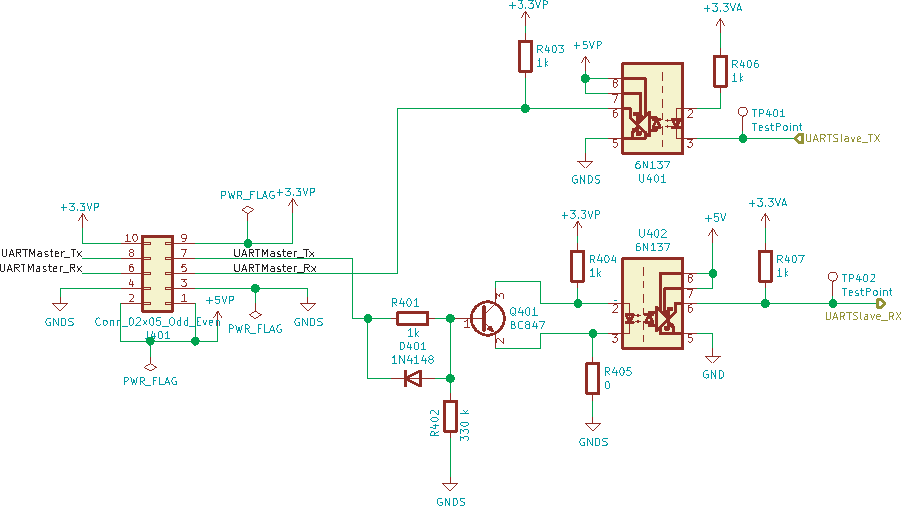
\includegraphics[width=1\textwidth]{./Figures/InterfazOpto.pdf}
	\caption{Diagrama esquematico de la interfaz UART optoaislada.}
	\label{fig:InterfazOpto}
\end{figure}


\subsection{Entradas y salidas digitales}

Del listado de requerimientos surge la necesidad de implementar tres entradas digitales, tres salidas digitales y una salida de alimentación para los módulos adicionales. La figura \ref{fig:EntradaDigital} muestra el diagrama esquemático del circuito adaptador de nivel de una de las entradas digitales la cual fue diseñada para tolerar niveles de tensión de hasta 30 V y proteger al microcontrolador STM32F108C8T6.

\begin{figure}[H]
	\centering
	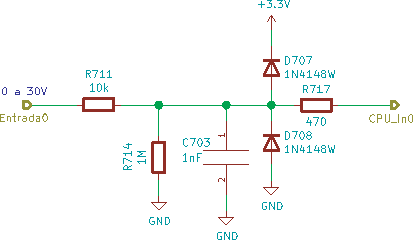
\includegraphics[width=0.8\textwidth]{./Figures/EntradaDigital.pdf}
	\caption{Diagrama esquematico de una entrada digital.}
	\label{fig:EntradaDigital}
\end{figure}

Para las salidas digitales se escogió una configuración de salida optoacoplada de colector abierto como se ve en la figura \ref{fig:SalidaDigital}. En esta misma figura, además, se puede ver la salida de alimentación de 220 VAC de los módulos adicionales, esta se implementó con una salida a relé de dos contactos que permite la conexión y desconexión de fase y neutro al mismo tiempo.

\begin{figure}[H]
	\centering
	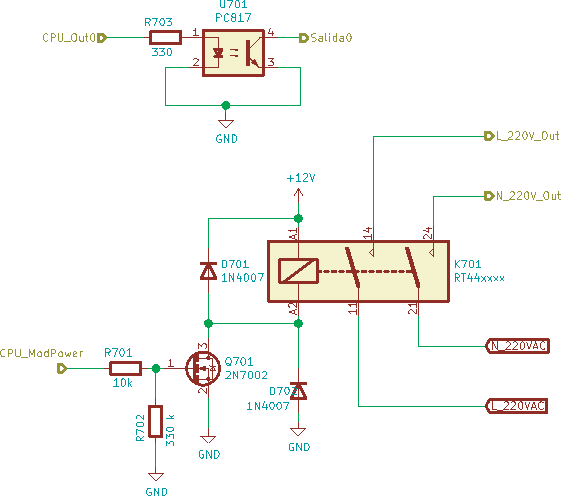
\includegraphics[width=0.8\textwidth]{./Figures/SalidaDigital.pdf}
	\caption{Diagrama esquemático de una salida digital y la salida de alimentacion de 220 VAC.}
	\label{fig:SalidaDigital}
\end{figure}

\subsection{Salida y entradas analogicas}

Cada puerto del módulo principal dispone de una salida analógica con capacidad de generar señales entre 0-10 V. Como el microcontrolador STM32F108C8T6 no posee un conversor digital analógico fue necesario utilizar un conversor externo, el conversor elegido para el diseño fue el MCP4725 de microchip. Este conversor de 12 bits y un canal se comunica con el microcontrolador mediante un bus I2C. 
Como se puede ver en el diagrama esquemático de la figura \ref{fig:SalidaAnalogica} se tuvo que diseñar una etapa de amplificación que lleve el nivel de tensión del rango 0 - 3.3 V que puede entregar el MCP4725 hasta el rango de 0 - 10 V que fue especificado en los requerimientos para la salida analógica..

\begin{figure}[H]
	\centering
	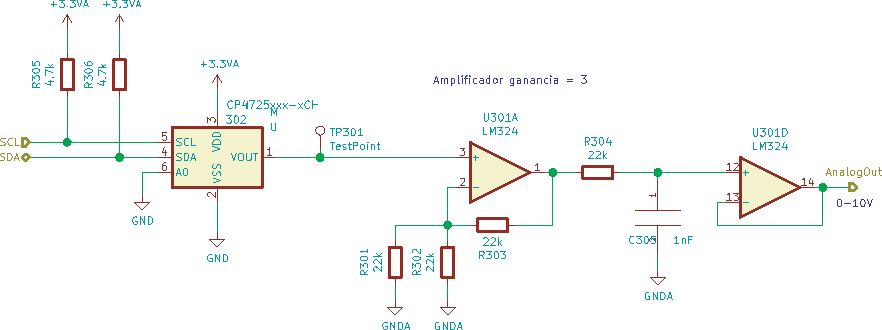
\includegraphics[width=1\textwidth]{./Figures/SalidaAnalogica.pdf}
	\caption{Diagrama esquemático de la salida analógica de un puerto.}
	\label{fig:SalidaAnalogica}
\end{figure}

Para las entradas analógicas se dio uso a los dos conversores analógico-digital incluidos en el microcontrolador STM32F103C8T6, que muestrean ambas entradas en forma simultanea. Al igual que la salida analogica, fue necesario hacer una adaptación del nivel de tensión de entrada de 0 -10 V al rango 0 - 3.3 V con un circuito atenuador y un buffer. En la figura \ref{fig:EntradaAnalogica} se puede ver el circuito atenuador implementado que además, para proteger al puerto, se diseño una protección por sobre tensión en la entrada analogica que limita la tensión a un máximo de 12 V.

\begin{figure}[H]
	\centering
	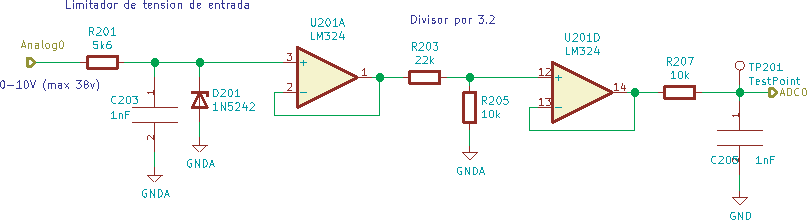
\includegraphics[width=1\textwidth]{./Figures/EntradaAnalogica.pdf}
	\caption{Diagrama esquemático de una entrada analógica.}
	\label{fig:EntradaAnalogica}
\end{figure}




\section{Desarrollo de hardware del módulo prueba de drivers}

El módulo test de drivers es un circuito diseñado para realizar la medición de los valores de tensión y corriente en la salida de un driver para iluminación LED. En el diagrama en bloques de la figura \ref{fig:BloquesTestDriver} se puede ver que el módulo está compuesto por cinco etapas que adaptan las señales a los niveles de tensión soportados por los puertos del módulo principal y la forma en que se conecta con el modulo principal y la carga.

\begin{figure}[H]
	\centering
	\includegraphics[width=1\textwidth]{./Figures/BloquesTestDriver.pdf}
	\caption{Diagrama en bloques del modulo prueba de drivers.}
	\label{fig:BloquesTestDriver}
\end{figure}


De las cinco etapas de este módulo, dos sirven para mediciones analogicas. La primera etapa, cuyo esquemático se puede ver en la figura \ref{fig:MedicionCorriente}, es para la medición de corriente de salida de drivers de LEDs. Esta se diseñó para hacer mediciones entre 0 y 2,5 A de corriente continua entregando a la salida un nivel de tensión proporcional en el rango 0 - 10 V.

\begin{figure}[H]
	\centering
	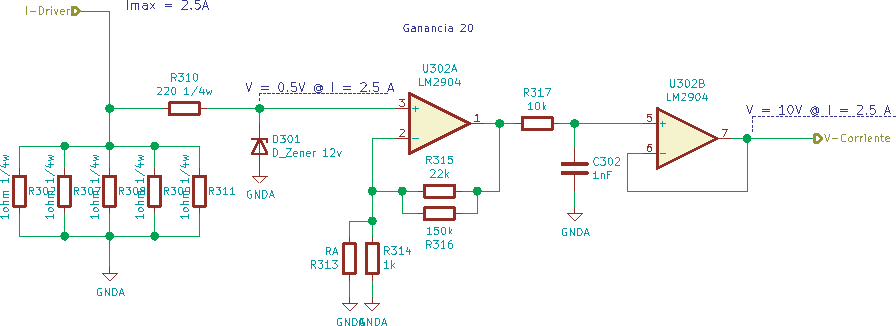
\includegraphics[width=1\textwidth]{./Figures/MedicionCorriente.pdf}
	\caption{Esquematico del circuito de medición de corriente de drivers.}
	\label{fig:MedicionCorriente}
\end{figure}

La segunda etapa de medicion analogica es una etapa de medicion de tension continua de la salida del driver de LEDs. En el esquemático de la figura \ref{fig:MedicionTension} se puede ver el circuito atenuador y separador diseñado para llevar el nivel de tensión del rango 0 - 500 VDC a 0 - 10 V compatible con los puertos del módulo principal.

\begin{figure}[H]
	\centering
	\includegraphics[width=0.7\textwidth]{./Figures/MedicionTension.pdf}
	\caption{Esquematico del circuito de medición de tensión de drivers.}
	\label{fig:MedicionTension}
\end{figure}

Este módulo además posee dos salidas para dimerizar drivers, una de ellas de dimerizado analogico, para la cual se construyo una etapa buffer de ganancia unitaria que separe al modulo principal del driver. La otra salida de dimerizado es una salida discreta que mediante la combinación de dos relés conmuta resistencias con las que se puede configurar el dimerizado en algunos modelos de drivers.
La última etapa de este módulo es una salida tipo on/off a relé para hacer la conexión y desconexión de la carga de los drivers de LEDs.


\section{Desarrollo de hardware del módulo prueba de temporizadores}

El moulo de prueba de temporizadores esta formado por dos etapas, la etapa de disparo y la etapa de captura de salida. En la figura \ref{fig:BloquesTestTemp} se puede ver el diagrama en bloques, la conexión con el modulo principal y con los dos tipos de temporizadores que soporta.


\begin{figure}[H]
	\centering
	\includegraphics[width=0.9\textwidth]{./Figures/BloquesTestTemp.pdf}
	\caption{Diagrama en bloques del módulo prueba de temporizadores.}
	\label{fig:BloquesTestTemp}
\end{figure}


\section{Desarrollo de circuitos impresos}

El diseño de los circuitos impresos y los diagramas esquemáticos se realizaron con el software libre KICAD. En total se diseñaron tres modelos, el circuito impreso de un puerto del modulo principal, que en la figura \ref{fig:FotoPuerto} se puede ver un renderizado del mismo junto con una foto de la placa real, el del modulo de prueba de drivers y el del modulo de prueba de temporizadores, que se pueden ver en la figura \ref{fig:ModulosAdic}. De cada uno se fabricaron seis unidades.


\begin{figure}[H]
  \centering
  \begin{subfigure}[b]{0.45\textwidth}
    \centering
     \includegraphics[width=0.9\textwidth]{./RenderPuerto.png}
     \centering
	\caption{\protect\raggedright Renderizado en Kicad.}
	\label{fig:Render}
  \end{subfigure}
  \hfill
  \begin{subfigure}[b]{0.45\textwidth}
    \centering
     \includegraphics[width=0.9\textwidth]{./FotoPuerto.jpg}
     \centering
	\caption{\protect\raggedright Foto real.}
	\label{fig:Foto}
  \end{subfigure}
	\caption{Renderizado y fotografía de placa de un puerto del módulo principal}
    \label{fig:FotoPuerto}
\end{figure}

\begin{figure}[H]
  \centering
  \begin{subfigure}[b]{0.45\textwidth}
    \centering
     \includegraphics[width=0.9\textwidth]{./FotoTestDriver.jpg}
     \centering
	\caption{\protect\raggedright Placa prueba de drivers.}
	\label{fig:PlacaDrivers}
  \end{subfigure}
  \hfill
  \begin{subfigure}[b]{0.45\textwidth}
    \centering
     \includegraphics[width=0.9\textwidth]{./FotoTestTemp.jpg}
     \centering
	\caption{\protect\raggedright Placa prueba de temporizadores.}
	\label{fig:PlacaTemp}
  \end{subfigure}
	\caption{Fotografía de la placa del módulo prueba de drivers de LEDs y la placa del módulo prueba de temporizadores de tres y cuatro terminales}
    \label{fig:ModulosAdic}
\end{figure}


% SOFTWARE
\section{Arquitectura del software}

Con la intención de facilitar al lector el entendimiento de la arquitectura del software implementado, se decidió seccionar la documentación según la plataforma de hardware en la que se ejecuta cada pieza de software. Siguiendo con este criterio podemos diferenciar tres secciones de software a analizar:
\begin{itemize}
	\item Software ejecutado en los módulos Bluepill STM32 de los puertos.
	\item Software ejecutado en la placa de desarrollo EDU-CIAA.
	\item Software ejecutado en la terminal de la interfaz web.
\end{itemize}
	
Cada una de estas secciones está comunicada a través de un medio físico y un protocolo. En la figura \ref{fig:ProtocolosComSoftware} se pueden ver estos módulos de software y el protocolo con el que se comunican.

\begin{figure}[H]
	\centering
	\includegraphics[width=0.9\textwidth]{./Figures/ProtocolosComSoftware.pdf}
	\caption{Protocolos de comunicación entre bloques de software}
	\label{fig:ProtocolosComSoftware}
\end{figure}

\subsection{Arquitectura del software ejecutado en los módulos Bluepill.}

El software que se ejecuta en el módulo Bluepill de desarrollo siguiendo una arquitectura tipo Interrupción. Esta arquitectura se utiliza en aplicaciones con eventos que deben ser atendidos en forma rápida y eficientemente y esto debe hacerse independientemente de lo que esté haciendo el sistema en ese momento.(1)
Teniendo en cuenta la arquitectura arquitectura elegida en esta aplicación podemos identificar un bloque de código principal que se ejecuta en un bucle infinito y dos interrupciones a atender, una de ellas es una interrupción temporal para el muestreo de señales analogicas y la otra está dada por el protocolo de la interfaz UART optoaislada, cuando el maestro genera una interrupción en el esclavo para comunicarse.
El diagrama en bloques de la figura \ref{fig:TareasSTM32} indica los segmentos de software que se desarrollaron bajo esta arquitectura y la forma en que se comunican entre sí.

\begin{figure}[H]
	\centering
	\includegraphics[width=0.9\textwidth]{./Figures/TareasSTM32.pdf}
	\caption{Diagrama en bloques general del software del módulo Bluepill.}
	\label{fig:TareasSTM32}
\end{figure}

\subsection{Implementación del software del módulo Bluepill.}
Para el desarrollo del software sobre el módulo Bluepill se escogió el entorno de desarrollo STM32CubeIDE de la empresa ST Microelectronics. Este entorno de desarrollo incorpora la herramienta gráfica STM32CubeMX utilizada para la configuración e inicialización de puertos, interrupciones y clock del procesador. Además STM32CubeIDE ofrece distintas bibliotecas de software, entre ellas la STM32Cube HAL(Hardware abstraction layer, capa de abstracción de hardware) que se utilizó para el manejo de los distintos periféricos del microcontrolador.

A continuación se hace un desglose de las funciones principales de los tres bloques de software del módulo Bluepill.
Funciones bucle principal:
\begin{itemize}
	\item Leer dirección del módulo
	\item Actualizar datos del DAC mediante el bus I2C.
	\item Actualizar salidas digitales.
\end{itemize}

Funciones interrupción por temporizador:
\begin{itemize}
	\item Actualizar el estado de las entradas digitales.
	\item Actualizar el estado de las entradas analogicas, colocar en buffer y calcular promedio.
	\item Armar la trama con los datos de entradas analogicas y digitales que se transmitirán por UART.
\end{itemize}

Funciones interrupción UART:
\begin{itemize}
	\item Identificar tramas que llegan por la UART y descartar las que no corresponden al módulo.
	\item Separar los datos recibidos para que el bucle principal los utilice.
	\item Transmitir por UART la trama formada en la interrupción del temporizador.
\end{itemize}


Funciones interrupción por temporizador:
\begin{itemize}
	\item Actualizar el estado de las entradas digitales.
	\item Actualizar el estado de las entradas analogicas, colocar en buffer y calcular promedio.
	\item Armar la trama con los datos de entradas analogicas y digitales que se transmitirán por UART.
\end{itemize}

Funciones interrupción UART:
\begin{itemize}
	\item Identificar tramas que llegan por la UART y descartar las que no corresponden al módulo.
	\item Separar los datos recibidos para que el bucle principal los utilice.
	\item Transmitir por UART la trama formada en la interrupción del temporizador.
\end{itemize}

En la figura \ref{fig:BloquesPrinTime} se muestra el diagrama en bloques del software implementado para el bucle principal y la interrupción del timer. Por otro lado el diagrama en bloques de la figura \ref{fig:BloquesUart} ayuda a comprender la implementacion del codigo \ref{cod:codigoUART} de la interrupción UART. Allí se puede ver como se realiza el procesamiento de cada byte que llega y asi separar las distintas partes de la trama.


\begin{lstlisting}[label=cod:codigoUART, caption= Codigo del callback de interrupción de recepción por UART.]
void HAL_UART_RxCpltCallback(UART_HandleTypeDef *UartHandle)
{
	uint8_t auxByte;
	//Si el primer bit es 1 significa que llego el primer byte de una trama
	if (bufferUARTin[receiveIndex]& 0x80){
		//Chequeo address del dato, si es el propio envio los datos de ADCs y entradas
		if (((auxByte=bufferUARTin[receiveIndex]>>4)&0x07)==moduleAddr){
			receiveIndex = 1;//Primer byte de la trama recibido
			for (auxByte=0; auxByte < OUTPUT_BUFFER_SIZE; auxByte++){
				bufferUARTout[auxByte] = packedDataOut [packedDataIndex][auxByte];
				}
			//Transmito la informacion por la UART
			if(HAL_UART_Transmit_IT(&huart1, bufferUARTout, OUTPUT_BUFFER_SIZE)!= HAL_OK){
				 Error_Handler();
			  }
		}
		else receiveIndex = 0; //Si el dato no corresponde a este address reinicio el indice
	}
	//Si el primer bit es 0 significa que llego el 2 o 3 byte puede o no ser para el address actual
	else{
		if (receiveIndex == 1){
			//Ordeno los datos para el DAC
			DACData[1] = bufferUARTin[1]<<2; 
			DACData[0] = ((bufferUARTin[0]&0x07)<<1)|(bufferUARTin[1]>>6); 
			receiveIndex = 2; //Segundo byte recibido
		}
		else
			if (receiveIndex == 2)			{
				//Ordeno los datos de las salidas digitales
				outData=bufferUARTin[2]|((bufferUARTin[0] & 0x08)<<4);
				dataFlag = 1; //Indico que hay datos para enviar al DAC y a las salidas digitales
				receiveIndex = 0; //Tercer byte recibido
			}
	}

	//Reinicio la recepcion de otro dato por UART y lo guardo en el buffer
	if(HAL_UART_Receive_IT(&huart1, (uint8_t*) &bufferUARTin[receiveIndex], 1) != HAL_OK){
	    Error_Handler();
	  }
}


\end{lstlisting}

\begin{figure}[ht]
	\centering
	\includegraphics[width=0.7\textwidth]{./Figures/BloquesUart.pdf}
	\caption{Diagrama en bloques de la interrupción de recepción por UART.}
	\label{fig:BloquesUart}
\end{figure}


\begin{figure}[H]
  \centering
  \begin{subfigure}[b]{0.45\textwidth}
    \centering
     \includegraphics[width=0.8\textwidth]{./BloquesMain.pdf}
     \centering
	\caption{\protect\raggedright Bucle principal.}
	\label{fig:BloquesMain}
  \end{subfigure}
  \hfill
  \begin{subfigure}[b]{0.45\textwidth}
    \centering
     \includegraphics[width=0.9\textwidth]{./BloquesTimer.pdf}
     \centering
	\caption{\protect\raggedright Timer.}
	\label{fig:BloquesTimer}
  \end{subfigure}
	\caption{Diagrama en bloques del bucle principal e interrupción del timer.}
    \label{fig:BloquesPrinTime}
\end{figure}


\subsection{Arquitectura del software ejecutado en la EDU-CIAA.}
\label{sec:ArqEDUCIAA}
Al momento de elegir la arquitectura del software que se iba a utilizar para esta seccion se realizo el siguiente listado de funciones que debian realizarse.
\begin{itemize}
	\item Montar un servido web para la interfaz de usuario.
	\item Correr una terminal para configuración.
	\item Ejecutar los test.
	\item Actualizar el estado de los puertos con una periodicidad de 1ms
\end{itemize}
En esta lista puede apreciarse que se trata de funciones o tareas de diversas características y complejidades que deben ejecutarse en paralelo y en tiempo real. Una forma de resolver este tipo de problemas es mediante el uso de sistemas operativos de tiempo real, es por ello que se escogió FreeRTOS como base para esta seccion de software.
Luego se pudo crear la estructura en capas de la figura \ref{fig:CapasCIAA} con capas de abstracción de hardware, entre las que se destaca la biblioteca sAPI en su versión 2, la capa del sitema operativo FreeRTOS, una capa de drivers propios y la capa de aplicación.

\begin{figure}[H]
	\centering
	\includegraphics[width=1\textwidth]{./Figures/CapasCIAA.pdf}
	\caption{Modelo de capas del software en la EDU-CIAA.}
	\label{fig:CapasCIAA}
\end{figure}

Analizando en detalle las capas de aplicación y drivers, se puede ver que se incluyeron cuatro bloques de drivers y nueve tareas que a continuación se describen brevemente.

Drivers
\begin{itemize}
	\item Driver de puertos: Este driver se desarrolló para comunicar la EDU-CIAA con los puertos de conexión vistos en la seccion \ref{sec:puertos} mediante el protocolo que se estableció para la interfaz UART optoaislada. El driver utiliza un timer del sistema operativo para realizar un polling a los puertos cada 1ms cumpliendo con los requerimientos de taza de muestreo muestreo. Además este driver utiliza colas dos colas por cada puerto, mediante las cuales lee los datos a transferir y envia los datos recibidos a las tareas que los requieran.
	\item Drive EEPROM: Se utiliza para separa, grabar y leer la memoria EEPROM propia del microcontrolador de la EDU-CIAA. En ella se guardan los parámetros de cada uno de los test y los datos de conexión de la red WIFI.
	\item Driver UART servidor web y terminal: Son dos instanciaciones del mismo módulos de software. Este driver se desarrollo para permitir la comunicación con la UART del modulo ESP-01 y y mediante el uso de colas evitar que el servidor web y la terminal produzcan un bloqueo de tareas.
\end{itemize}
	
Tareas
\begin{itemize}
	\item Terminal: Consiste en una interfaz de usuario básica que utiliza la UART-USB que posee la EDU-CIAA unicamente destinada a la configuración de la red WIFI y al debugging.
Servidor web: Realiza la configuración y control del modulo ESP-01 para la conexión a la red WIFI, el reconocimiento de peticiones HTTP, envia comandos al interprete y envia las respuestas HTTP. 
	\item Interprete: Esta tarea se ocupa de interpretar y ejecutar los comandos que llegan de la interfaz de usuario a través del servidor web y además recopila y empaqueta los datos de estado de las pruebas que el servidor web envia a la interfaz de usuario.
	\item Test 0 - 5: Las seis tareas test son propiamente el software de prueba. Allí residen los distintos tipos de pruebas que se pueden realizar. Cada una de estas tareas esta asociada a un solo puerto del modulo principal al que puede controlar.
\end{itemize}	
	
El esquema de la figura \ref{fig:ComuTareas} detalla el modo en que se comunican las distintas tareas que se ejecutan sobre el sistema operativo.

\begin{figure}[H]
	\centering
	\includegraphics[width=1\textwidth]{./Figures/ComuTareas.pdf}
	\caption{Esquema de comunicación entre tareas.}
	\label{fig:ComuTareas}
\end{figure}



\subsection{Tarea terminal}

La tarea terminal fue diseñada con el fin de interpretar comandos recibidos mediante una UART y ejecutarlos. Por tratarse de una interfaz únicamente pensada para la configuración de la conexión a la red WIFI, el set de comandos aceptados se reduce a:
\begin{itemize}
	\item SSID: Devuelve la identificación SSID actual de la red. También acepta un parámetro opcional para modificar la SSID. Ejemplo: SSID RedFiuba, actualiza el SSID de la red a la que se debe conectar a RedFiuba.
	\item PASS: Modifica la contraseña de la red. Requiere de un parámetro a continuación que es la contraseña que se desea configurar.
	\item WIIP: Devuelve la dirección IP actual del dispositivo en la red. También acepta un parámetro opcional para modificar la IP. Ejemplo: WIIP 192.168.0.1, fuerza la IP a la dirección 192.168.0.1.
	\item RECN: Indica al servidor web que debe iniciar un proceso de reconexión, es necesario ejecutar este comando luego de modificar alguno de los parámetros de conexión a la red.
\end{itemize}	

El funcionamiento de esta tarea fue diagramado en cuatro etapa:
\begin{itemize}
	\item Recibir datos y crear hash del comando
	\item Identificar comando
	\item Capturar parámetro
	\item Ejecutar el comando
\end{itemize}	

La forma que se escogió para hacer el hash consiste en construir una variable de 32 bits con cuatro bytes donde la posición de cada byte en dicha variable corresponde al orden en que los bytes llegaron por la UART asignada a la terminal. Cada vez que llega un caracter por la UART este desplaza a los anteriores y elimina al más viejo formando un nuevo hash que debe ser identificado, luego capturado el parámetro si hubiese y ejecutado.


\subsection{Tarea servidor web}

En el desarrollo del servidor web se utilizó como base la biblioteca ESP8266 incluida en la sAPI, que permite mediante comandos AT la configuración del módulo ESP-01 y la comunicación utilizando el protocolo HTTP con la interfaz de usuario en un navegador web. Fue necesario adaptar la biblioteca para lo cual se sustituyeron las  funciones originales para recepción de datos de la UART por funciones del driver UART propio que evita el bloqueo de tareas.
Además se agregaron funciones y servicios que se detallan a continuación.
\begin{itemize}
	\item Configuración de IP: Se incorporó la opción de configurar el del modulo ESP-01 mediante el comando AT+CIPSTA.
	\item Parseo request: Se amplió la capacidad de parseo de las request HTTP para identificar el método y el cuerpo.
	\item Request GET: Se amplió el soporte de la request con métodos GET permitiendo que la carga de la página web de la interfaz de usuario se haga por partes y actualice los datos en pantalla sin necesidad de cargar la página web completa.
	\item Request POST: Se dio soporte al método POST para enviar datos y órdenes desde la interfaz de usuario a la aplicación.
\end{itemize}

El diagrama en bloques de la figura \ref{fig:BloquesServidor} permite comprender el funcionamiento del servidor web implementado. En este diagrama se puede ver que el servidor inicia con un proceso de configuración y conexión a la red y luego se mantiene en un lazo en el que espera peticiones y las responde.
Por otro lado la figura \ref{fig:TransaccionesHTTP} muestra un diagrama de transacciones típico para la carga de la página web de interfaz de usuario, en el se puede observar que una vez transferidos todos los datos para construir la página web, solo es necesario hacer peticiones HTTP del tipo GET /data a las que el servidor responde con los datos de estado de las pruebas en formato JSON y finalmente el navegador actualiza la información en pantalla.

\begin{figure}[H]
	\centering
	\includegraphics[width=0.3\textwidth]{./Figures/BloquesServidor.pdf}
	\caption{Diagrama en bloques del servidor web.}
	\label{fig:BloquesServidor}
\end{figure}

\begin{figure}[H]
	\centering
	\includegraphics[width=0.6\textwidth]{./Figures/TransaccionesHTTP.pdf}
	\caption{DIagrama de transiciones entre el servidor web y el navegador.}
	\label{fig:TransaccionesHTTP}
\end{figure}

\subsection{Tarea intérprete}
Esta sección describe detalladamente el desarrollo realizado para implementar las funciones de la tarea intérprete que fueron descritas en la sección \ref{sec:ArqEDUCIAA}.
Una de las funciones que el intérprete debe realizar es la de interpretar y ejecutar comandos provenientes del servidor web. En rigor estos comandos son el resultado de peticiones HTTP con método POST que envía el navegador web donde corre la interfaz de usuario. Estas peticiones pueden cambiar el estado de una o más pruebas, pueden cambiar el tipo de prueba en curso o enviar datos de configuración de las pruebas.
Luego la secuencia puede resumirse en:
\begin{itemize}
	\item Se genera la petición HTTP POST accediendo a un recurso.
	\item El servidor traduce la petición en un comando para el intérprete y lo coloca en una cola de comandos.
	\item El intérprete captura el comando de la cola, lo interpreta y lo ejecuta.
\end{itemize}

Todos los comandos que recibe el intérprete están asociados a eventos producidos al presionar un botón de la interfaz de usuario. Estos se pueden clasificar de la siguiente forma.
Comandos de botones de base
Son comandos que se producen al presionar alguno de los botones de la base de la interfaz de usuario comunes a todos los tipos de pruebas. Estos son:
\begin{itemize}
	\item Panel anterior: Implica cambiar al tipo de prueba anterior.
	\item Panel siguiente: Implica cambiar al tipo de prueba posterior.
	\item Detener Pruebas: Detiene todas las pruebas en curso.
\end{itemize}
Comandos de botones de panel
Son comandos originados al presionar alguno de los botones del panel en la interfaz de usuario en una prueba en particular. Los comandos disponibles son:
\begin{itemize}
	\item Marcha/Parada: Al recibir este comando el intérprete debe alternar el estado de la prueba. Si estaba en curso la detiene y si estaba detenida la inicia.
	\item Guardar: Este comando detiene todas la pruebas en curso y guarda los parámetros recibidos para la configuración del test.	
\end{itemize}

La otra función que realiza el intérprete es la de recopilar el estado de cada una de las pruebas, accediendo sus respectivas estructuras de estados, y formar una cadena en formato JSON con estos datos para que esté disponible cuando el servidor web la requiera.
La forma de esta cadena se puede ver en el código \ref{cod:cadenaJSON}

\begin{lstlisting}[label=cod:cadenaJSON, caption= Cadena de datos de panel en notación JSON.]
   "panel":N de panel,
   "data":[
      Estado (test 1),
      Marcha/Parada (test 1),
      Pasa/No pasa (test 1),
      Parametro/Medicion 0 (test 1),
      Parametro/Medicion 1 (test 1),
      Parametro/Medicion 2 (test 1),
      Parametro/Medicion 3 (test 1),
      Guardar (test 1),
			.
			.
			.
      Estado (test N),
      Marcha/Parada (test N),
      Pasa/No pasa (test N),
      Parametro/Medicion 0 (test N),
      Parametro/Medicion 1 (test N),
      Parametro/Medicion 2 (test N),
      Parametro/Medicion 3 (test N),
      Guardar (test N),
   ]

\end{lstlisting}


\subsection{Tareas test}

Las tareas test son las responsables de controlar los puertos y ejecutar las distintas secuencias de prueba. Cada una de las seis tareas test es una instanciación de un mismo algoritmo. En el código \ref{cod:crearTest} se presenta una porción del algoritmo donde se crean las tareas test que ejecutan la misma función testTask y a cada una de estas tareas se le asigna una estructura FSMRegister del tipo testStatet cuya definición se puede ver en el código \ref{cod:estTestState}.
Esta estructura contiene todas las variables asociadas al estado de la prueba, los parámetros de configuración, resultados, la cola de entrada de instrucciones del intérprete y el puerto del módulo principal que fue asignado a dicha tarea.


\begin{lstlisting}[label=cod:crearTest, caption= Algoritmo de creación de tareas test.]
//Inicializar el vector de datos y comunicacion de los tests
	for (i=0;i<PORTS_NUMBER;i++)
	{
		FSMRegisters[i].port = ports.port[i]; //Asignar colas del puerto
		FSMRegisters[i].test = 0;
		FSMRegisters[i].state = INIT;
		//Creo la cola por donde llegan las ordenes para la tarea de pruebas
		FSMRegisters[i].testControlQueue = xQueueCreate(CONTROL_QUEUE_LEN,sizeof(testOrder_t)); 


		//Creo la tarea de la prueba y le paso el registro de datos
		xTaskCreate(
			testsTask,                // Funcion de la tarea
			(const char *)"Test",     
			configMINIMAL_STACK_SIZE, 
			(void*)&FSMRegisters[i],  // Registro de estado de la tarea.
			tskIDLE_PRIORITY+1,         
			0                           
		);
	}


\end{lstlisting}

\begin{lstlisting}[label=cod:estTestState, caption= Estructura de estado del test.]
typedef struct
{
	uint8_t test; 		//Test en curso
	uint8_t state; 		//Estado
	uint32_t result[RESULT_NUM]; //resultados de la prueba
	uint8_t pasa; 		//Pasa o no pasa
	uint32_t *param;	//parametros de la prueba ( entrada)
	QueueHandle_t testControlQueue; //Cola de instrucciones
	portsData_t port;	//Puerto


	//Variables para calculos intermedios
	uint8_t i;			// numero de iteracion
	uint8_t adcSamples; //numero de samples de ADC
	uint32_t tickRegister;	//Captura del Tick counter.
	uint32_t ADC_1; //Suma de muestras CH0
	uint32_t ADC_2; //Suma de muestras CH1
	//Entradas digitales
	uint16_t  in0Sum; 
	uint16_t  in1Sum;
	uint16_t  in2Sum;

} testState_t;
\end{lstlisting}

A través de la cola de instrucciones, el intérprete puede enviar órdenes a la tarea test. Esta ordenes están compuestas de dos parámetros: prueba a realizar y estado de la prueba que se desea forzar. De los posibles estados de las pruebas el intérprete sólo utiliza dos start y stop.
En cuanto a los tipos de pruebas se implementaron dos, una para prueba de temporizadores y una para prueba de drivers. Además se desarrolló una tercera opción para la calibración de la prueba de drivers que únicamente presenta en pantalla las mediciones de los ADC.
Cada una de las pruebas se desarrolló mediante máquinas de estados finitos (MEF). 
El diagrama de la figura \ref{fig:FSMTestDrivers} es una representación de la máquina de estados implementada para la prueba de drivers. A continuación se describen cada uno de sus estados
\begin{itemize}
	\item Init: En este estado se inicializan la salida analogica y todas las salidas digitales del puerto asignado a un valor que garantice la manipulación segura del equipo  a probar. Aquí se espera hasta que llegue la instrucción de iniciar. El mensaje en pantalla es INICIO.
	\item Start: Se configura el nivel de dimerizado. Por este estado se pasa tres veces para realizar mediciones con tres niveles de dimerización. El mensaje en pantalla es Probando.
	\item PoweOn: Activa la alimentación y espera 5 segundos a que el driver se estabilice.
	\item Measure: Luego de que el driver se estabilizó se hacen las mediciones de tensión y corriente. Aquí también se evalúan las mediciones. El mensaje en pantalla es Probando.
	\item Stop: Al igual que el estado Init se llevan todas las salidas del puerto a condición segura, pero en este estado el mensaje en pantalla es FIN.
\end{itemize}
	
\begin{figure}[H]
	\centering
	\includegraphics[width=1\textwidth]{./Figures/FSMTestDrivers.pdf}
	\caption{Diagrama de estados de la MEF del test de drivers.}
	\label{fig:FSMTestDrivers}
\end{figure}


En el caso de la prueba de temporizadores la máquina de estados implementada puede resumirse en los siguientes estados:
\begin{itemize}
	\item Init: Inicializa todas las salidas en un valor seguro para la operación por parte del usuario. El mensaje en pantalla es INICIO.
	\item Start: Se alimenta al equipo bajo prueba. El mensaje en pantalla es Configurar temporizador.
	\item Trigger: genera un pulso de disparo del temporizador. El mensaje en pantalla es Probando.
	\item WaitON: Se espera a que el temporizador se encienda durante treinta segundos. El mensaje en pantalla es Probando.
	\item WaitOFF: Se espera a que el temporizador se apague durante el tiempo máximo configurado en pantalla.
	\item CheckTime: Se evalúa el tiempo medido. El mensaje en pantalla es Probando.
	\item Stop: Se llevan las salidas al valor seguro de operación. El mensaje en pantalla es FIN.
\end{itemize}

Todos estos estados y sus transiciones pueden verse en el diagrama de la figura \ref{fig:FSMTestTemp}.

\begin{figure}[H]
	\centering
	\includegraphics[width=1\textwidth]{./Figures/FSMTestTemp.pdf}
	\caption{Diagrama de estados de la MEF del test de temporizadores.}
	\label{fig:FSMTestTemp}
\end{figure}

\subsection{Interfaz de usuario}

La interfaz de usuario es el medio por el cual el operario puede controlar el equipo probador.
Esta interfaz fue desarrollada de acuerdo con el requisito de que fuera accesible mediante un navegador web utilizando un dispositivo conectado a la misma red.
Por tratarse de una interfaz que se presenta como una página web fue necesario el uso de las tecnologías de desarrollo propias de la plataforma. En particular las dos tecnologías que más se utilizaron fueron JavaScript y HTML, en las que no se tenía ninguna experiencia antes de realizar el trabajo.
Desde el inicio del desarrollo, la página web de la interfaz, fue pensada para funcionar en forma de bloques, de modo que no fuera necesario cargar toda la página cada vez que algún valor indicado cambiase. Así se resolvió hacer un seccionamiento en tres partes:

\begin{itemize}
	\item Base: En la base se encuentran los botones de control comunes a todas las pruebas. La figura XXX es una captura de la base de la interfaz en el navegador web y se pueden ver el botón Detener Pruebas, los botones Panel anterior y panel siguiente y la indicación del panel actual. Cada uno de estos botones al ser presionados le indican al servidor , mediante una petición HTTP, que debe producirse una acción. Cada una de estas acciones ya fue descrita en la sección \ref{fig:Base}.
	\item Panel: El panel es el espacio donde se visualizan todas la indicaciones de estado y los parámetros de configuración de la prueba en curso. Aquí también se ubican los botones de Marcha/Parada y Guardar. Existe un panel distinto para cada tipo de prueba. Las figuras \ref{fig:PanelDriver}, \ref{fig:PanelTemp} y \ref{fig:PanelCal} son capturas de los paneles de las pruebas de drivers, temporizadores y el panel de calibración de ADCs respectivamente.

	\item Datos: Toda la información sobre el estado de las pruebas y los parámetros de configuración son recibidos por separado del panel y la base. Estos datos, que el servidor envía en formato JSON, son solicitados periódicamente y lograr así un refresco cada un segundo.
\end{itemize}

En la sección xxx se vio el proceso de carga de la página web desde el lado del servidor. Si se analiza del lado del navegador web se puede reconocer la siguiente secuencia:

\begin{itemize}
	\item El navegador solicita la página web mediante la petición GET / .
	\item El servidor responde con una página web en blanco, un conjunto de scripts para la carga de las distintas secciones y una instrucción inicial de ejecutar el script de carBody().
	\item Al ejecutar el script carBody() se crea un objeto XMLHttpRequest para enviar una petición HTTP GET /body, a la que el servidor responde con la sección Base de la interfaz.
	\item Una vez cargada la Base se ejecuta el script carPan() que envía la petición GET /panel. A esta petición el servidor responde con el panel correspondiente al test actual.
	\item Una vez cargado el panel, crea un timer de 1 segundo que periódicamente ejecuta el script carDat(). Este script envía la petición GET /data al servidor, que responde con los datos del panel actual. Luego se actualizan los datos en pantalla.
\end{itemize}

\begin{figure}[H]
	\centering
	\includegraphics[width=0.8\textwidth]{./Figures/Base.png}
	\caption{Captura de la base de la interfaz de usuario.}
	\label{fig:Base}
\end{figure}

\begin{figure}[H]
	\centering
	\includegraphics[width=0.7\textwidth]{./Figures/PanelDriver.png}
	\caption{Captura del panel de test de drivers.}
	\label{fig:PanelDriver}
\end{figure}

\begin{figure}[H]
	\centering
	\includegraphics[width=0.7\textwidth]{./Figures/PanelTemp.png}
	\caption{Captura del panel de test de temporizadores.}
	\label{fig:PanelTemp}
\end{figure}

\begin{figure}[H]
	\centering
	\includegraphics[width=0.7\textwidth]{./Figures/PanelCal.png}
	\caption{Captura del panel de calibracion de ADCs.}
	\label{fig:PanelCal}
\end{figure}